\section{问题描述}
本节我们对拆分学习中底部模型产生的拆分层表征带来的对顶部模型以及标签的隐私泄漏问题(模型补全攻击)进行描述和定义,并且将该隐私泄漏问题转化为一个攻击者的有监督或无监督的学习问题。

\begin{figure}[h!]
    \centering
    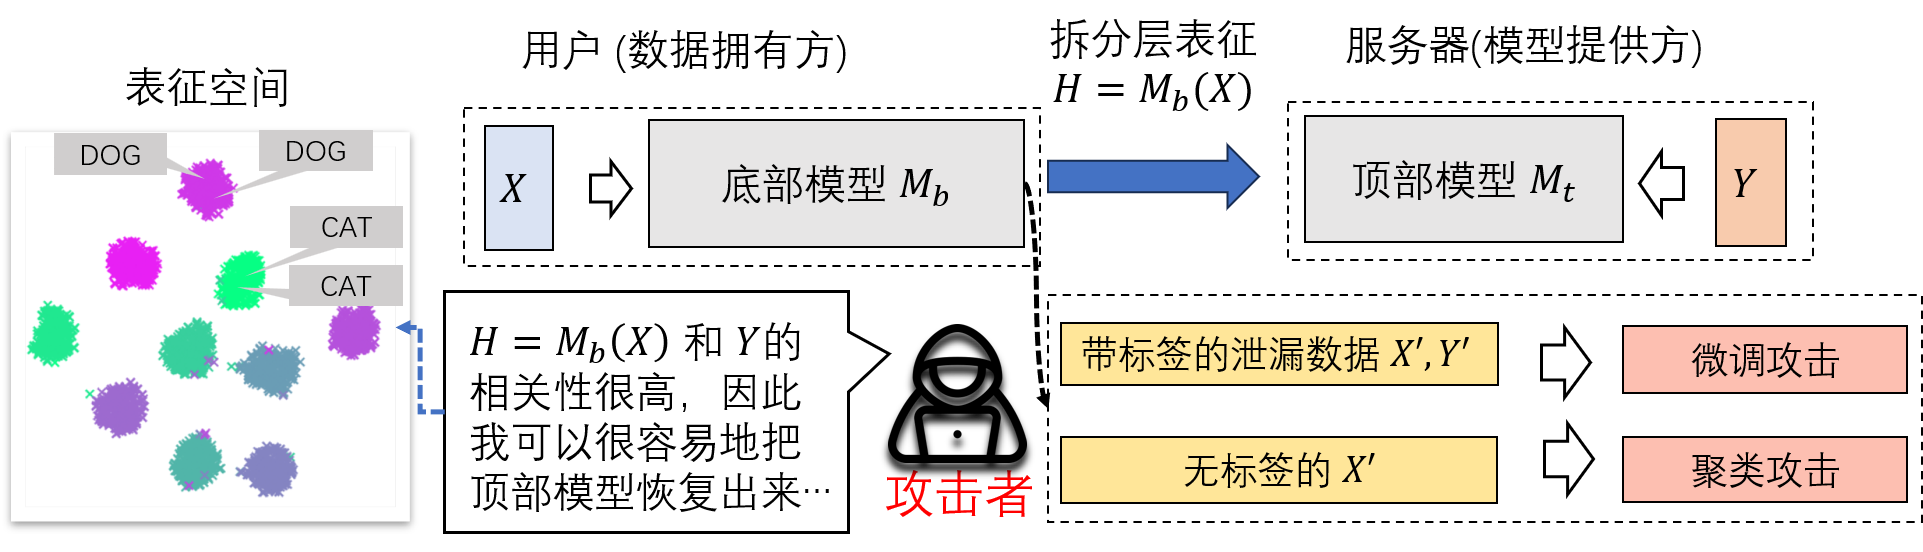
\includegraphics[width=1\linewidth]{Z_Resources/peloss_attack.png}
    \caption{拆分学习中底部模型带来的隐私泄露问题和模型补全攻击示意图}
    \label{fig:peloss:attack}
\end{figure}

\subsection{拆分层的隐私泄露}
许多对神经网络隐层进行可视化的研究都揭露了如下的规律:在神经网络的训练过程中,隐层表征与样本标签的关联性逐渐增加,相同标签对应的隐层表征会逐渐聚集成簇,而不同标签对应的隐层表征会逐渐分离开~\cite{paulo2017visualize_hidden,pezzotti2017deepeyes,cantareira2020hidden_vector_fields}。
%
并且位置越靠后的隐层的表征,与样本标签的关联性越高。
%
尽管上述的“同类别隐层表征靠近,不同类别隐层表征分离”的规律是神经网络具备学习能力的一个必需原因,这个规律给拆分学习带来了很大的隐私泄漏风险。
%

理想的两方拆分学习$X \stackrel{M_b}{\to} H \stackrel{M_t}{\to} Y$应该满足下述的两个条件:
\begin{itemize}
    \item 从$H$推出$X$是困难的,从而保证用户的输入数据的隐私。
    \item 从$H$推出$Y$是困难的,因此用户必须和模型拥有方合作,才能获取模型预测值,而不能仅仅通过$M_b$获取预测值,从而保证模型的隐私。
\end{itemize}
然而,前面所述的神经网络隐层表征的性质,恰恰说明$H$推出$Y$可能是十分容易的,与我们期望的理想拆分学习的性质所矛盾。
%
假设攻击者腐化了用户,它可以轻松地通过少量带标签样本$(\cdots, (X_i, Y_i), \cdots)$,然后通过用户侧的底部模型$M_b$来产生拆分层表征$(\cdots, H_i, \cdots)$,并通过拆分层表征-标签对$(\cdots, (H_i, Y_i), \cdots)$来训练顶部模型$M_t$,从而窃取整个模型;
同时,攻击者也可以直接通过无标签的样本产生大量表征,并对其进行聚类得到类别标签,从而得到样本标签$Y$或训练出顶部模型$M_t$。
%
我们将这两种攻击统称为模型补全攻击(Model Completion Attack),与现有研究一致。
%
\autoref{fig:peloss:attack}是模型补全攻击的示意图。


\subsection{威胁模型}
为了更清晰地定义上述的隐私泄漏问题,我们定义两种攻击方法:
\begin{itemize}
    \item \textbf{微调攻击}:
    假设攻击者具有底部模型$M_b$,并且拥有少部分泄露的带标签样本$Z = (\cdots, (X'_i, Y'_i), \cdots)$,其中每一种类别的样本都有$k$个。攻击者也知道顶部模型$M_t$的结构,但是不知道具体参数。
    攻击者通过$(\cdots, (X'_i, Y'_i), \cdots)$和固定的$M_b$来微调$M_t$,从而实现窃取模型的目的。

    \item \textbf{聚类攻击}:
    假设攻击者具有底部模型$M_b$,并且拥有大量泄漏的无标签样本$X = (\cdots, X_i, \cdots)$。
    攻击者通过底部模型产生中间表征$H = (\cdots, H_i, \cdots)$,然后对其进行聚类产生类别标签,使得聚类模型实现顶部模型$M_t$的功能,从而实现窃取整体模型的目的。
\end{itemize}

注意到,我们的攻击场景设定为拆分学习的推断阶段而非训练阶段,因为本文的目标是降低拆分层表征的隐私泄露。
%
如果要对拆分层梯度进行保护,可以使用非敏感数据集进行训练,或者使用基于密码学的隐私保护神经网络训练方法~\cite{mohassel2017secureml,wagh2019securenn}。
%
除此之外,一些研究也指出对于无标签的样本进行无监督学习也能产生一个表现良好的分类模型~\cite{berthelot2019mixmatch,xuyi2021dp_ssl}。
但是这些方法与拆分学习无关,因为它们不需要任何关于底部模型或是拆分层表征的知识。
本文不对这些方法进行讨论。
%

\subsection{问题定义}
表面上看来,上述的攻击和模型正常的训练过程的目标是类似的:两者都会学习从拆分层表征$H$到标签$Y$的映射。
%
然而攻击者的训练过程和正常的模型训练过程存在着一个本质区别,即两者的训练数据不同。
正常的模型训练工程需要大量的带标签数据,而在模型补全攻击中,我们假设攻击者只能获取少量的带标签样本。
%
因此,我们可以把模型补全攻击转化成一个机器学习问题。
具体而言,防御的目标转换为:控制底部模型$M_b$,使得整体模型$(M_b, M_t)$有较高的准确率,但是使用少量带标签的$H = M_b(X)$对随机初始化的$M_t$进行微调,则会产生较高的泛化误差。
%

\begin{definition}[底部模型优势]
    我们定义底部模型优势为攻击者利用底部模型$M_b$进行攻击产生的额外优势。
    考虑一个攻击者$\mathcal A$和其输入数据$D$以及底部模型$M_b$(可以为空),其输出则为一个完全模型$M = (M_b, M_t): X \to Y$,底部模型优势可以定义为:
    \begin{equation}
        Adv(M_b; \mathcal A) = \mathbb E_D \{ R[\mathcal A(D; null)] - R[\mathcal A(D; M_b)]\},
    \end{equation}
    其中,$R[\cdot]$ 表示攻击者产生的完全模型在测试集上的误差,$\mathcal A(D; null)$ 表示攻击者在没有底部模型时的产生的完全模型。
\end{definition}
%
例如,在微调攻击时,$D = (\cdots, (X_i, Y_i), \cdots)$ 是泄露的带标签的样本;而在聚类攻击时,$D = (\cdots, X_i, \cdots)$是泄露的无标签的样本。
%
而$\mathcal A(D; null)$相当于攻击者在没有任何底部模型信息,仅有泄露数据的情况下产生的完全模型,即使用带标签数据/无标签数据从零开始训练模型(Train from Scratch)。

\begin{definition}[完美保护]
    对于某种攻击$\mathcal A$,如果底部模型$M_b$满足底部模型优势$Adv(M_b, \mathcal A) \le 0$,则称$M_b$对$\mathcal A$产生了完美保护,因为$M_b$的存在对攻击效果的提升没有任何作用。
\end{definition}

基于以上定义,本文目标可以描述为训练一个拆分学习模型$(M_b, M_t)$使得:
\begin{itemize}
    \item 模型本身的准确率越高越好。
    \item 底部模型针对于微调攻击和聚类攻击的底部模型优势越小越好。
\end{itemize}